\documentclass[a4paper,12pt]{article}

\usepackage[utf8x]{inputenc}
\usepackage[T2A]{fontenc}
\usepackage[english, russian]{babel}

% Опционно, требует  apt-get install scalable-cyrfonts.*
% и удаления одной строчки в cyrtimes.sty
% Сточку не удалять!
% \usepackage{cyrtimes}

% Картнки и tikz
\usepackage{graphicx}
\usepackage{tikz}
\usetikzlibrary{snakes,arrows,shapes}


% Некоторая русификация.
\usepackage{misccorr}
\usepackage{indentfirst}
\renewcommand{\labelitemi}{\normalfont\bfseries{--}}

% Увы, поля придётся уменьшить из-за листингов.
\topmargin -1cm
\oddsidemargin -0.5cm
\evensidemargin -0.5cm
\textwidth 17cm
\textheight 24cm

\sloppy

% Оглавление в PDF
\usepackage[
bookmarks=true,
colorlinks=true, linkcolor=black, anchorcolor=black, citecolor=black, menucolor=black,filecolor=black, urlcolor=black,
unicode=true
]{hyperref}

% Для исходного кода в тексте
\newcommand{\Code}[1]{\texttt{#1}}


\title{Отчёт по лабораторной работе \\ <<Механизмы протокола TCP>>}
\author{Ермаков М.С. ИУ7-31М}

\begin{document}

\maketitle

\tableofcontents

% Текст отчёта должен быть читаемым!!! Написанное здесь является рыбой.

\section{Установка и разрыв соединения}

Вывод tcpdump с c2 при установке соединения от c1 до c6:
\begin{Verbatim}
14:36:28.003927 IP 10.10.0.2.36912 > 10.50.0.2.1996: Flags [S], seq 2237042055, win 64240, options [mss 1460,sackOK,TS val 1256467007 ecr 0,nop,wscale 7], length 0
14:36:28.004191 IP 10.50.0.2.1996 > 10.10.0.2.36912: Flags [S.], seq 1393844325, ack 2237042056, win 65160, options [mss 536,sackOK,TS val 2060647298 ecr 1256467007,nop,wscale 7], length 0
14:36:28.004273 IP 10.10.0.2.36912 > 10.50.0.2.1996: Flags [.], ack 1, win 502, options [nop,nop,TS val 1256467007 ecr 2060647298], length 0
\end{Verbatim}

Вывод tcpdump с c3 c включенным MSS clamp при установке соединения от c1 до c6:
\begin{Verbatim}
14:36:28.003979 IP 10.10.0.2.36912 > 10.50.0.2.1996: Flags [S], seq 2237042055, win 64240, options [mss 1460,sackOK,TS val 1256467007 ecr 0,nop,wscale 7], length 0
14:36:28.004168 IP 10.50.0.2.1996 > 10.10.0.2.36912: Flags [S.], seq 1393844325, ack 2237042056, win 65160, options [mss 536,sackOK,TS val 2060647298 ecr 1256467007,nop,wscale 7], length 0
14:36:28.004290 IP 10.10.0.2.36912 > 10.50.0.2.1996: Flags [.], ack 1, win 502, options [nop,nop,TS val 1256467007 ecr 2060647298], length 0
\end{Verbatim}

Вывод tcpdump с c2 при закрытии соединения на c1:
\begin{Verbatim}
14:43:08.035884 IP 10.10.0.2.36912 > 10.50.0.2.1996: Flags [F.], seq 8, ack 8, win 502, options [nop,nop,TS val 1256867039 ecr 2061037865], length 0
14:43:08.036067 IP 10.50.0.2.1996 > 10.10.0.2.36912: Flags [F.], seq 8, ack 9, win 510, options [nop,nop,TS val 2061047330 ecr 1256867039], length 0
14:43:08.036111 IP 10.10.0.2.36912 > 10.50.0.2.1996: Flags [.], ack 9, win 502, options [nop,nop,TS val 1256867039 ecr 2061047330], length 0
\end{Verbatim}

Вывод tcpdump с c3 c включенным MSS clamp при закрытии соединения на c1:
\begin{Verbatim}
14:43:08.035905 IP 10.10.0.2.36912 > 10.50.0.2.1996: Flags [F.], seq 8, ack 8, win 502, options [nop,nop,TS val 1256867039 ecr 2061037865], length 0
14:43:08.036050 IP 10.50.0.2.1996 > 10.10.0.2.36912: Flags [F.], seq 8, ack 9, win 510, options [nop,nop,TS val 2061047330 ecr 1256867039], length 0
14:43:08.036120 IP 10.10.0.2.36912 > 10.50.0.2.1996: Flags [.], ack 9, win 502, options [nop,nop,TS val 1256867039 ecr 2061047330], length 0
\end{Verbatim}

Как видно выше, при установке соединения выставляется MSS равный 536 байтам, это максимальный размер полезной нагрузки одного ip пакета на маршруте от c1 до c6.

\section{Окно получателя}

Вывод tcpdump на c3 при отправке сообщений от c1 до c4:
\begin{Verbatim}
15:06:34.229374 IP 10.30.0.2.3002 > 10.10.0.2.46370: Flags [.], ack 1001, win 504, options [nop,nop,TS val 984938323 ecr 2662916011], length 0
15:06:34.229521 IP 10.30.0.2.3002 > 10.10.0.2.46370: Flags [.], ack 2001, win 500, options [nop,nop,TS val 984938323 ecr 2662916011], length 0
15:06:34.229665 IP 10.30.0.2.3002 > 10.10.0.2.46370: Flags [.], ack 3001, win 496, options [nop,nop,TS val 984938323 ecr 2662916011], length 0
15:06:34.229805 IP 10.30.0.2.3002 > 10.10.0.2.46370: Flags [.], ack 4001, win 492, options [nop,nop,TS val 984938323 ecr 2662916011], length 0
15:06:34.230055 IP 10.30.0.2.3002 > 10.10.0.2.46370: Flags [.], ack 5001, win 488, options [nop,nop,TS val 984938324 ecr 2662916012], length 0
15:06:34.230182 IP 10.30.0.2.3002 > 10.10.0.2.46370: Flags [.], ack 6001, win 484, options [nop,nop,TS val 984938324 ecr 2662916012], length 0
15:06:34.230585 IP 10.30.0.2.3002 > 10.10.0.2.46370: Flags [.], ack 7001, win 480, options [nop,nop,TS val 984938324 ecr 2662916012], length 0
15:06:34.230597 IP 10.30.0.2.3002 > 10.10.0.2.46370: Flags [.], ack 8573, win 474, options [nop,nop,TS val 984938324 ecr 2662916012], length 0
15:06:34.230602 IP 10.30.0.2.3002 > 10.10.0.2.46370: Flags [.], ack 11193, win 464, options [nop,nop,TS val 984938324 ecr 2662916012], length 0
15:06:34.230791 IP 10.30.0.2.3002 > 10.10.0.2.46370: Flags [.], ack 13289, win 456, options [nop,nop,TS val 984938324 ecr 2662916012], length 0
15:06:34.230803 IP 10.30.0.2.3002 > 10.10.0.2.46370: Flags [.], ack 16433, win 443, options [nop,nop,TS val 984938324 ecr 2662916012], length 0
15:06:34.230808 IP 10.30.0.2.3002 > 10.10.0.2.46370: Flags [.], ack 21673, win 423, options [nop,nop,TS val 984938324 ecr 2662916012], length 0
15:06:34.231048 IP 10.30.0.2.3002 > 10.10.0.2.46370: Flags [.], ack 25865, win 406, options [nop,nop,TS val 984938325 ecr 2662916013], length 0
15:06:34.231059 IP 10.30.0.2.3002 > 10.10.0.2.46370: Flags [.], ack 32153, win 382, options [nop,nop,TS val 984938325 ecr 2662916013], length 0
15:06:34.231063 IP 10.30.0.2.3002 > 10.10.0.2.46370: Flags [.], ack 42633, win 341, options [nop,nop,TS val 984938325 ecr 2662916013], length 0
15:06:34.231284 IP 10.30.0.2.3002 > 10.10.0.2.46370: Flags [.], ack 43681, win 337, options [nop,nop,TS val 984938325 ecr 2662916013], length 0
15:06:34.273719 IP 10.30.0.2.3002 > 10.10.0.2.46370: Flags [.], ack 86649, win 163, options [nop,nop,TS val 984938367 ecr 2662916013,nop,nop,sack 1 {86125:86649}], length 0
15:06:34.316939 IP 10.30.0.2.3002 > 10.10.0.2.46370: Flags [.], ack 107513, win 82, options [nop,nop,TS val 984938410 ecr 2662916055,nop,nop,sack 1 {107085:107513}], length 0
15:06:34.350386 IP 10.30.0.2.3002 > 10.10.0.2.46370: Flags [.], ack 118009, win 41, options [nop,nop,TS val 984938444 ecr 2662916099,nop,nop,sack 1 {117993:118009}], length 0
15:06:34.387303 IP 10.30.0.2.3002 > 10.10.0.2.46370: Flags [.], ack 122805, win 4, options [nop,nop,TS val 984938481 ecr 2662916132,nop,nop,sack 1 {122281:122805}], length 0
15:06:34.610564 IP 10.30.0.2.3002 > 10.10.0.2.46370: Flags [.], ack 123317, win 0, options [nop,nop,TS val 984938704 ecr 2662916392], length 0
15:06:34.850354 IP 10.30.0.2.3002 > 10.10.0.2.46370: Flags [.], ack 123317, win 0, options [nop,nop,TS val 984938944 ecr 2662916392], length 0
15:06:36.183937 IP 10.30.0.2.3002 > 10.10.0.2.46370: Flags [.], ack 123317, win 0, options [nop,nop,TS val 984940278 ecr 2662916392], length 0
15:06:36.230025 IP 10.30.0.2.3002 > 10.10.0.2.46370: Flags [R.], seq 1, ack 123317, win 508, options [nop,nop,TS val 984940324 ecr 2662916392], length 0
\end{Verbatim}

Вывод tcpdump на c4 при отправке сообщений на localhost:3002:
\begin{Verbatim}
15:43:46.379309 IP 127.0.0.1.3002 > 127.0.0.1.45882: Flags [S.], seq 1852601175, ack 1646362229, win 65483, options [mss 65495,sackOK,TS val 154535886 ecr 154535886,nop,wscale 7], length 0
15:43:46.379510 IP 127.0.0.1.3002 > 127.0.0.1.45882: Flags [.], ack 1001, win 504, options [nop,nop,TS val 154535886 ecr 154535886], length 0
15:43:46.379563 IP 127.0.0.1.3002 > 127.0.0.1.45882: Flags [.], ack 2001, win 500, options [nop,nop,TS val 154535886 ecr 154535886], length 0
15:43:46.379605 IP 127.0.0.1.3002 > 127.0.0.1.45882: Flags [.], ack 3001, win 496, options [nop,nop,TS val 154535886 ecr 154535886], length 0
15:43:46.379636 IP 127.0.0.1.3002 > 127.0.0.1.45882: Flags [.], ack 4001, win 492, options [nop,nop,TS val 154535886 ecr 154535886], length 0
15:43:46.379670 IP 127.0.0.1.3002 > 127.0.0.1.45882: Flags [.], ack 5001, win 488, options [nop,nop,TS val 154535886 ecr 154535886], length 0
15:43:46.379713 IP 127.0.0.1.3002 > 127.0.0.1.45882: Flags [.], ack 6001, win 484, options [nop,nop,TS val 154535886 ecr 154535886], length 0
15:43:46.379750 IP 127.0.0.1.3002 > 127.0.0.1.45882: Flags [.], ack 7001, win 480, options [nop,nop,TS val 154535886 ecr 154535886], length 0
15:43:46.379782 IP 127.0.0.1.3002 > 127.0.0.1.45882: Flags [.], ack 8001, win 476, options [nop,nop,TS val 154535886 ecr 154535886], length 0
15:43:46.379813 IP 127.0.0.1.3002 > 127.0.0.1.45882: Flags [.], ack 9001, win 472, options [nop,nop,TS val 154535886 ecr 154535886], length 0
15:43:46.379852 IP 127.0.0.1.3002 > 127.0.0.1.45882: Flags [.], ack 10001, win 468, options [nop,nop,TS val 154535887 ecr 154535886], length 0
15:43:46.379895 IP 127.0.0.1.3002 > 127.0.0.1.45882: Flags [.], ack 11001, win 465, options [nop,nop,TS val 154535887 ecr 154535887], length 0
15:43:46.387132 IP 127.0.0.1.3002 > 127.0.0.1.45882: Flags [.], ack 12001, win 461, options [nop,nop,TS val 154535894 ecr 154535887], length 0
15:43:46.387147 IP 127.0.0.1.3002 > 127.0.0.1.45882: Flags [.], ack 44742, win 333, options [nop,nop,TS val 154535894 ecr 154535887], length 0
15:43:46.387170 IP 127.0.0.1.3002 > 127.0.0.1.45882: Flags [.], ack 77483, win 78, options [nop,nop,TS val 154535894 ecr 154535894], length 0
15:43:46.593629 IP 127.0.0.1.3002 > 127.0.0.1.45882: Flags [.], ack 87467, win 0, options [nop,nop,TS val 154536100 ecr 154536100], length 0
15:43:46.800009 IP 127.0.0.1.3002 > 127.0.0.1.45882: Flags [.], ack 87467, win 0, options [nop,nop,TS val 154536307 ecr 154536100], length 0
15:43:48.053268 IP 127.0.0.1.3002 > 127.0.0.1.45882: Flags [.], ack 87467, win 0, options [nop,nop,TS val 154537560 ecr 154536100], length 0
15:43:48.379981 IP 127.0.0.1.3002 > 127.0.0.1.45882: Flags [R.], seq 1, ack 87467, win 512, options [nop,nop,TS val 154537887 ecr 154536100], length 0
\end{Verbatim}

\section{Окно отправителя}

\begin{Verbatim}
root@c1:~# ./nagle nodelay 10.40.0.2 1996 1 20
root@c2:/# tcpdump -n tcp
\end{Verbatim}

\begin{Verbatim}
tcpdump: verbose output suppressed, use -v or -vv for full protocol decode
listening on eth0, link-type EN10MB (Ethernet), capture size 262144 bytes
17:49:20.598392 IP 10.10.0.2.51538 > 10.40.0.2.1996: Flags [S], seq 597974571, win 64240, options [mss 1460,sackOK,TS val 2973171331 ecr 0,nop,wsc
ale 7], length 0
17:49:20.698633 IP 10.40.0.2.1996 > 10.10.0.2.51538: Flags [S.], seq 3561072669, ack 597974572, win 65160, options [mss 1460,sackOK,TS val 3908486
058 ecr 2973171331,nop,wscale 7], length 0
17:49:20.698712 IP 10.10.0.2.51538 > 10.40.0.2.1996: Flags [.], ack 1, win 502, options [nop,nop,TS val 2973171431 ecr 3908486058], length 0
17:49:20.698878 IP 10.10.0.2.51538 > 10.40.0.2.1996: Flags [P.], seq 1:101, ack 1, win 502, options [nop,nop,TS val 2973171432 ecr 3908486058], le
ngth 100
17:49:20.700097 IP 10.10.0.2.51538 > 10.40.0.2.1996: Flags [P.], seq 101:201, ack 1, win 502, options [nop,nop,TS val 2973171433 ecr 3908486058],
length 100
17:49:20.701353 IP 10.10.0.2.51538 > 10.40.0.2.1996: Flags [P.], seq 201:301, ack 1, win 502, options [nop,nop,TS val 2973171434 ecr 3908486058],
length 100
17:49:20.702622 IP 10.10.0.2.51538 > 10.40.0.2.1996: Flags [P.], seq 301:401, ack 1, win 502, options [nop,nop,TS val 2973171435 ecr 3908486058],
length 100
17:49:20.703794 IP 10.10.0.2.51538 > 10.40.0.2.1996: Flags [P.], seq 401:501, ack 1, win 502, options [nop,nop,TS val 2973171436 ecr 3908486058],
length 100
17:49:20.705043 IP 10.10.0.2.51538 > 10.40.0.2.1996: Flags [P.], seq 501:601, ack 1, win 502, options [nop,nop,TS val 2973171438 ecr 3908486058],
length 100
17:49:20.706189 IP 10.10.0.2.51538 > 10.40.0.2.1996: Flags [P.], seq 601:701, ack 1, win 502, options [nop,nop,TS val 2973171439 ecr 3908486058],
length 100
17:49:20.707431 IP 10.10.0.2.51538 > 10.40.0.2.1996: Flags [P.], seq 701:801, ack 1, win 502, options [nop,nop,TS val 2973171440 ecr 3908486058],
length 100
17:49:20.708541 IP 10.10.0.2.51538 > 10.40.0.2.1996: Flags [P.], seq 801:901, ack 1, win 502, options [nop,nop,TS val 2973171441 ecr 3908486058],
length 100
17:49:20.709975 IP 10.10.0.2.51538 > 10.40.0.2.1996: Flags [P.], seq 901:1001, ack 1, win 502, options [nop,nop,TS val 2973171442 ecr 3908486058],
length 100
17:49:20.722945 IP 10.10.0.2.51538 > 10.40.0.2.1996: Flags [FP.], seq 1001:2001, ack 1, win 502, options [nop,nop,TS val 2973171456 ecr 3908486058
], length 1000
17:49:20.799031 IP 10.40.0.2.1996 > 10.10.0.2.51538: Flags [.], ack 101, win 509, options [nop,nop,TS val 3908486159 ecr 2973171432], length 0
17:49:20.799124 IP 10.40.0.2.1996 > 10.10.0.2.51538: Flags [P.], seq 1:101, ack 101, win 509, options [nop,nop,TS val 3908486159 ecr 2973171432], length 100
17:49:20.799241 IP 10.10.0.2.51538 > 10.40.0.2.1996: Flags [R], seq 597974672, win 0, length 0
17:49:20.800228 IP 10.40.0.2.1996 > 10.10.0.2.51538: Flags [.], ack 201, win 509, options [nop,nop,TS val 3908486160 ecr 2973171433], length 0
17:49:20.800290 IP 10.10.0.2.51538 > 10.40.0.2.1996: Flags [R], seq 597974772, win 0, length 0
17:49:20.801470 IP 10.40.0.2.1996 > 10.10.0.2.51538: Flags [.], ack 301, win 509, options [nop,nop,TS val 3908486161 ecr 2973171434], length 0
17:49:20.801521 IP 10.10.0.2.51538 > 10.40.0.2.1996: Flags [R], seq 597974872, win 0, length 0
17:49:20.802715 IP 10.40.0.2.1996 > 10.10.0.2.51538: Flags [.], ack 401, win 509, options [nop,nop,TS val 3908486162 ecr 2973171435], length 0
17:49:20.802761 IP 10.10.0.2.51538 > 10.40.0.2.1996: Flags [R], seq 597974972, win 0, length 0
17:49:20.803855 IP 10.40.0.2.1996 > 10.10.0.2.51538: Flags [.], ack 501, win 509, options [nop,nop,TS val 3908486163 ecr 2973171436], length 0
17:49:20.803897 IP 10.10.0.2.51538 > 10.40.0.2.1996: Flags [R], seq 597975072, win 0, length 0
17:49:20.805110 IP 10.40.0.2.1996 > 10.10.0.2.51538: Flags [.], ack 601, win 509, options [nop,nop,TS val 3908486165 ecr 2973171438], length 0
17:49:20.805152 IP 10.10.0.2.51538 > 10.40.0.2.1996: Flags [R], seq 597975172, win 0, length 0
17:49:20.806370 IP 10.40.0.2.1996 > 10.10.0.2.51538: Flags [.], ack 701, win 509, options [nop,nop,TS val 3908486166 ecr 2973171439], length 0
17:49:20.806384 IP 10.10.0.2.51538 > 10.40.0.2.1996: Flags [R], seq 597975272, win 0, length 0
17:49:20.807585 IP 10.40.0.2.1996 > 10.10.0.2.51538: Flags [.], ack 801, win 509, options [nop,nop,TS val 3908486167 ecr 2973171440], length 0
17:49:20.807599 IP 10.10.0.2.51538 > 10.40.0.2.1996: Flags [R], seq 597975372, win 0, length 0
17:49:20.808624 IP 10.40.0.2.1996 > 10.10.0.2.51538: Flags [.], ack 901, win 509, options [nop,nop,TS val 3908486168 ecr 2973171441], length 0
17:49:20.808646 IP 10.10.0.2.51538 > 10.40.0.2.1996: Flags [R], seq 597975472, win 0, length 0
17:49:20.810359 IP 10.40.0.2.1996 > 10.10.0.2.51538: Flags [.], ack 1001, win 509, options [nop,nop,TS val 3908486170 ecr 2973171442], length 0
17:49:20.810407 IP 10.10.0.2.51538 > 10.40.0.2.1996: Flags [R], seq 597975572, win 0, length 0
17:49:20.823237 IP 10.40.0.2.1996 > 10.10.0.2.51538: Flags [.], ack 2002, win 502, options [nop,nop,TS val 3908486183 ecr 2973171456], length 0
17:49:20.823246 IP 10.40.0.2.1996 > 10.10.0.2.51538: Flags [.], seq 101:1549, ack 2002, win 502, options [nop,nop,TS val 3908486183 ecr 2973171456], length 1448
17:49:20.823271 IP 10.10.0.2.51538 > 10.40.0.2.1996: Flags [R], seq 597976573, win 0, length 0
17:49:20.823274 IP 10.10.0.2.51538 > 10.40.0.2.1996: Flags [R], seq 597976573, win 0, length 0
17:49:20.823300 IP 10.40.0.2.1996 > 10.10.0.2.51538: Flags [FP.], seq 1549:2001, ack 2002, win 502, options [nop,nop,TS val 3908486183 ecr 2973171456], length 452
17:49:20.823308 IP 10.10.0.2.51538 > 10.40.0.2.1996: Flags [R], seq 597976573, win 0, length 0
\end{Verbatim}

Опыт неверный, так как окно отправителя нельзя точно узнать через tcpdump, потому что программа не показывает еще неотправленные данные в буффере клиента. Получается можно посчитать только не что уже были отправлены и не подтверждены, в случае выше, размер окна тогда растет от 0 байт до 2000.

\begin{figure}
\centering
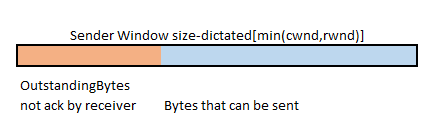
\includegraphics{sender_congestion_window.png}
\caption{Размер окна отправителя}
\label{fig:sender_congestion_window}
\end{figure}

\section{Нейгл и Мишналь}

%Мы должны увидеть, что мы посылаем неполный сегмент, как только подтверждены все неполные сегменты (даже если полные не подтверждены).

\begin{Verbatim}
root@c1:~# ./nagle default 10.40.0.2 1996 0 30
root@c2:/# tcpdump -n tcp
\end{Verbatim}

\begin{Verbatim}
18:13:33.738109 IP 10.10.0.2.51916 > 10.40.0.2.1996: Flags [S], seq 2335795120, win 64240, options [mss 1460,sackOK,TS val 2974624471 ecr 0,nop,wscale 7], length 0
18:13:33.838229 IP 10.40.0.2.1996 > 10.10.0.2.51916: Flags [S.], seq 3199249179, ack 2335795121, win 65160, options [mss 1460,sackOK,TS val 3909939198 ecr 2974624471,nop,wscale 7], length 0
18:13:33.838262 IP 10.10.0.2.51916 > 10.40.0.2.1996: Flags [.], ack 1, win 502, options [nop,nop,TS val 2974624571 ecr 3909939198], length 0
18:13:33.838332 IP 10.10.0.2.51916 > 10.40.0.2.1996: Flags [P.], seq 1:101, ack 1, win 502, options [nop,nop,TS val 2974624571 ecr 3909939198], length 100
18:13:33.839191 IP 10.10.0.2.51916 > 10.40.0.2.1996: Flags [.], seq 101:1549, ack 1, win 502, options [nop,nop,TS val 2974624572 ecr 3909939198], length 1448
18:13:33.839986 IP 10.10.0.2.51916 > 10.40.0.2.1996: Flags [.], seq 1549:2997, ack 1, win 502, options [nop,nop,TS val 2974624573 ecr 3909939198], length 1448
18:13:33.840137 IP 10.10.0.2.51916 > 10.40.0.2.1996: Flags [FP.], seq 2997:3001, ack 1, win 502, options [nop,nop,TS val 2974624573 ecr 3909939198], length 4
18:13:33.938699 IP 10.40.0.2.1996 > 10.10.0.2.51916: Flags [.], ack 101, win 509, options [nop,nop,TS val 3909939298 ecr 2974624571], length 0
18:13:33.938708 IP 10.40.0.2.1996 > 10.10.0.2.51916: Flags [P.], seq 1:101, ack 101, win 509, options [nop,nop,TS val 3909939298 ecr 2974624571], length 100
18:13:33.938741 IP 10.10.0.2.51916 > 10.40.0.2.1996: Flags [R], seq 2335795221, win 0, length 0
18:13:33.939229 IP 10.40.0.2.1996 > 10.10.0.2.51916: Flags [.], ack 1549, win 501, options [nop,nop,TS val 3909939299 ecr 2974624572], length 0
18:13:33.939249 IP 10.10.0.2.51916 > 10.40.0.2.1996: Flags [R], seq 2335796669, win 0, length 0
18:13:33.939264 IP 10.40.0.2.1996 > 10.10.0.2.51916: Flags [P.], seq 101:1549, ack 1549, win 501, options [nop,nop,TS val 3909939299 ecr 2974624572], length 1448
18:13:33.939270 IP 10.10.0.2.51916 > 10.40.0.2.1996: Flags [R], seq 2335796669, win 0, length 0
18:13:33.940155 IP 10.40.0.2.1996 > 10.10.0.2.51916: Flags [.], ack 2997, win 501, options [nop,nop,TS val 3909939300 ecr 2974624573], length 0
18:13:33.940161 IP 10.40.0.2.1996 > 10.10.0.2.51916: Flags [P.], seq 1549:2997, ack 2997, win 501, options [nop,nop,TS val 3909939300 ecr 2974624573], length 1448
18:13:33.940177 IP 10.10.0.2.51916 > 10.40.0.2.1996: Flags [R], seq 2335798117, win 0, length 0
18:13:33.940179 IP 10.10.0.2.51916 > 10.40.0.2.1996: Flags [R], seq 2335798117, win 0, length 0
18:13:33.940232 IP 10.40.0.2.1996 > 10.10.0.2.51916: Flags [FP.], seq 2997:3001, ack 3002, win 501, options [nop,nop,TS val 3909939300 ecr 2974624573], length 4
18:13:33.940238 IP 10.10.0.2.51916 > 10.40.0.2.1996: Flags [R], seq 2335798122, win 0, length 0
\end{Verbatim}

Выше видно что данные накапливаются в буффере перед отправкой и отправляется сегмент размером в MSS.

\section{Аггрессивная буферизация}

\begin{Verbatim}
root@c1:~# ./nagle cork 10.40.0.2 1996 -1 10
root@c2:/# tcpdump -n tcp
\end{Verbatim}

\begin{Verbatim}
18:25:10.211530 IP 10.10.0.2.51950 > 10.40.0.2.1996: Flags [S], seq 2475327219, win 64240, options [mss 1460,sackOK,TS val 2975320944 ecr 0,nop,wscale 7], length 0
18:25:10.311873 IP 10.40.0.2.1996 > 10.10.0.2.51950: Flags [S.], seq 1775870978, ack 2475327220, win 65160, options [mss 1460,sackOK,TS val 3910635671 ecr 2975320944,nop,wscale 7], length 0
18:25:10.311905 IP 10.10.0.2.51950 > 10.40.0.2.1996: Flags [.], ack 1, win 502, options [nop,nop,TS val 2975321045 ecr 3910635671], length 0
18:25:10.312057 IP 10.10.0.2.51950 > 10.40.0.2.1996: Flags [FP.], seq 1:1001, ack 1, win 502, options [nop,nop,TS val 2975321045 ecr 3910635671], length 1000
18:25:10.412473 IP 10.40.0.2.1996 > 10.10.0.2.51950: Flags [.], ack 1002, win 502, options [nop,nop,TS val 3910635772 ecr 2975321045], length 0
18:25:10.412482 IP 10.40.0.2.1996 > 10.10.0.2.51950: Flags [P.], seq 1:513, ack 1002, win 502, options [nop,nop,TS val 3910635772 ecr 2975321045], length 512
18:25:10.412484 IP 10.40.0.2.1996 > 10.10.0.2.51950: Flags [FP.], seq 513:1001, ack 1002, win 502, options [nop,nop,TS val 3910635772 ecr 2975321045], length 488
18:25:10.412531 IP 10.10.0.2.51950 > 10.40.0.2.1996: Flags [R], seq 2475328221, win 0, length 0
18:25:10.412535 IP 10.10.0.2.51950 > 10.40.0.2.1996: Flags [R], seq 2475328221, win 0, length 0
\end{Verbatim}

Клиент отправляет по 100 байт за раз и данные буфферизируются.

\section{Отправка без задержки}

\begin{Verbatim}
root@c1:~# ./nagle nodelay 10.40.0.2 1996 -1 1000
root@c2:/# tcpdump -n tcp
\end{Verbatim}

\begin{Verbatim}
18:29:27.790919 IP 10.10.0.2.51964 > 10.40.0.2.1996: Flags [S], seq 4008017495, win 64240, options [mss 1460,sackOK,TS val 2975578524 ecr 0,nop,ws
cale 7], length 0
18:29:27.891041 IP 10.40.0.2.1996 > 10.10.0.2.51964: Flags [S.], seq 3264066248, ack 4008017496, win 65160, options [mss 1460,sackOK,TS val 391089
3251 ecr 2975578524,nop,wscale 7], length 0
18:29:27.891083 IP 10.10.0.2.51964 > 10.40.0.2.1996: Flags [.], ack 1, win 502, options [nop,nop,TS val 2975578624 ecr 3910893251], length 0
18:29:27.891151 IP 10.10.0.2.51964 > 10.40.0.2.1996: Flags [P.], seq 1:101, ack 1, win 502, options [nop,nop,TS val 2975578624 ecr 3910893251], le
ngth 100
18:29:27.891171 IP 10.10.0.2.51964 > 10.40.0.2.1996: Flags [P.], seq 101:201, ack 1, win 502, options [nop,nop,TS val 2975578624 ecr 3910893251],
length 100
18:29:27.891181 IP 10.10.0.2.51964 > 10.40.0.2.1996: Flags [P.], seq 201:301, ack 1, win 502, options [nop,nop,TS val 2975578624 ecr 3910893251],
length 100
18:29:27.891197 IP 10.10.0.2.51964 > 10.40.0.2.1996: Flags [P.], seq 301:401, ack 1, win 502, options [nop,nop,TS val 2975578624 ecr 3910893251],
length 100
18:29:27.891206 IP 10.10.0.2.51964 > 10.40.0.2.1996: Flags [P.], seq 401:501, ack 1, win 502, options [nop,nop,TS val 2975578624 ecr 3910893251],
length 100
18:29:27.891221 IP 10.10.0.2.51964 > 10.40.0.2.1996: Flags [P.], seq 501:601, ack 1, win 502, options [nop,nop,TS val 2975578624 ecr 3910893251],
length 100
18:29:27.891235 IP 10.10.0.2.51964 > 10.40.0.2.1996: Flags [P.], seq 601:701, ack 1, win 502, options [nop,nop,TS val 2975578624 ecr 3910893251],
length 100
18:29:27.891254 IP 10.10.0.2.51964 > 10.40.0.2.1996: Flags [P.], seq 701:801, ack 1, win 502, options [nop,nop,TS val 2975578624 ecr 3910893251],
length 100
18:29:27.891264 IP 10.10.0.2.51964 > 10.40.0.2.1996: Flags [P.], seq 801:901, ack 1, win 502, options [nop,nop,TS val 2975578624 ecr 3910893251],
length 100
18:29:27.891277 IP 10.10.0.2.51964 > 10.40.0.2.1996: Flags [P.], seq 901:1001, ack 1, win 502, options [nop,nop,TS val 2975578624 ecr 3910893251],
length 100
18:29:27.991257 IP 10.40.0.2.1996 > 10.10.0.2.51964: Flags [.], ack 101, win 509, options [nop,nop,TS val 3910893351 ecr 2975578624], length 0
18:29:27.991268 IP 10.40.0.2.1996 > 10.10.0.2.51964: Flags [.], ack 201, win 509, options [nop,nop,TS val 3910893351 ecr 2975578624], length 0
18:29:27.991271 IP 10.40.0.2.1996 > 10.10.0.2.51964: Flags [P.], seq 1:201, ack 201, win 509, options [nop,nop,TS val 3910893351 ecr 2975578624],
length 200
18:29:27.991272 IP 10.40.0.2.1996 > 10.10.0.2.51964: Flags [.], ack 301, win 509, options [nop,nop,TS val 3910893351 ecr 2975578624], length 0
18:29:27.991273 IP 10.40.0.2.1996 > 10.10.0.2.51964: Flags [.], ack 401, win 509, options [nop,nop,TS val 3910893351 ecr 2975578624], length 0
18:29:27.991324 IP 10.10.0.2.51964 > 10.40.0.2.1996: Flags [P.], seq 1001:3897, ack 1, win 502, options [nop,nop,TS val 2975578724 ecr 3910893351]
, length 2896
18:29:27.991328 IP 10.10.0.2.51964 > 10.40.0.2.1996: Flags [P.], seq 3897:6793, ack 1, win 502, options [nop,nop,TS val 2975578724 ecr 3910893351]
, length 2896
18:29:27.991330 IP 10.10.0.2.51964 > 10.40.0.2.1996: Flags [.], ack 201, win 501, options [nop,nop,TS val 2975578724 ecr 3910893351], length 0
18:29:27.991363 IP 10.40.0.2.1996 > 10.10.0.2.51964: Flags [.], ack 501, win 509, options [nop,nop,TS val 3910893351 ecr 2975578624], length 0
18:29:27.991366 IP 10.40.0.2.1996 > 10.10.0.2.51964: Flags [.], ack 601, win 509, options [nop,nop,TS val 3910893351 ecr 2975578624], length 0
18:29:27.991367 IP 10.40.0.2.1996 > 10.10.0.2.51964: Flags [.], ack 701, win 509, options [nop,nop,TS val 3910893351 ecr 2975578624], length 0
18:29:27.991368 IP 10.40.0.2.1996 > 10.10.0.2.51964: Flags [.], ack 801, win 509, options [nop,nop,TS val 3910893351 ecr 2975578624], length 0
18:29:27.991368 IP 10.40.0.2.1996 > 10.10.0.2.51964: Flags [.], ack 901, win 509, options [nop,nop,TS val 3910893351 ecr 2975578624], length 0
18:29:27.991369 IP 10.40.0.2.1996 > 10.10.0.2.51964: Flags [.], ack 1001, win 509, options [nop,nop,TS val 3910893351 ecr 2975578624], length 0
18:29:27.991392 IP 10.10.0.2.51964 > 10.40.0.2.1996: Flags [P.], seq 6793:9689, ack 201, win 501, options [nop,nop,TS val 2975578724 ecr 391089335
1], length 2896
18:29:27.991395 IP 10.10.0.2.51964 > 10.40.0.2.1996: Flags [P.], seq 9689:12585, ack 201, win 501, options [nop,nop,TS val 2975578724 ecr 39108933
51], length 2896
18:29:27.991568 IP 10.10.0.2.51964 > 10.40.0.2.1996: Flags [P.], seq 12585:15481, ack 201, win 501, options [nop,nop,TS val 2975578724 ecr 3910893
351], length 2896
18:29:27.991574 IP 10.10.0.2.51964 > 10.40.0.2.1996: Flags [P.], seq 15481:18377, ack 201, win 501, options [nop,nop,TS val 2975578724 ecr 3910893
351], length 2896
18:29:27.991575 IP 10.10.0.2.51964 > 10.40.0.2.1996: Flags [R.], seq 18377, ack 201, win 501, options [nop,nop,TS val 2975578724 ecr 3910893351],
length 0
18:29:28.091413 IP 10.40.0.2.1996 > 10.10.0.2.51964: Flags [.], ack 3897, win 496, options [nop,nop,TS val 3910893451 ecr 2975578724], length 0
18:29:28.091420 IP 10.40.0.2.1996 > 10.10.0.2.51964: Flags [.], ack 6793, win 485, options [nop,nop,TS val 3910893451 ecr 2975578724], length 0
18:29:28.091421 IP 10.40.0.2.1996 > 10.10.0.2.51964: Flags [P.], seq 201:1001, ack 6793, win 485, options [nop,nop,TS val 3910893451 ecr 297557872
4], length 800
18:29:28.091422 IP 10.40.0.2.1996 > 10.10.0.2.51964: Flags [.], seq 1001:2449, ack 6793, win 485, options [nop,nop,TS val 3910893451 ecr 297557872
4], length 1448
18:29:28.091450 IP 10.10.0.2.51964 > 10.40.0.2.1996: Flags [R], seq 4008021392, win 0, length 0
18:29:28.091453 IP 10.10.0.2.51964 > 10.40.0.2.1996: Flags [R], seq 4008024288, win 0, length 0
18:29:28.091454 IP 10.10.0.2.51964 > 10.40.0.2.1996: Flags [R], seq 4008024288, win 0, length 0
18:29:28.091485 IP 10.40.0.2.1996 > 10.10.0.2.51964: Flags [.], seq 3897:5345, ack 6793, win 485, options [nop,nop,TS val 3910893451 ecr 297557872
4], length 1448
18:29:28.091488 IP 10.40.0.2.1996 > 10.10.0.2.51964: Flags [.], seq 8241:9689, ack 12585, win 485, options [nop,nop,TS val 3910893451 ecr 2975578724], length 1448
18:29:28.091519 IP 10.10.0.2.51964 > 10.40.0.2.1996: Flags [R], seq 4008024288, win 0, length 0
18:29:28.091521 IP 10.10.0.2.51964 > 10.40.0.2.1996: Flags [R], seq 4008024288, win 0, length 0
18:29:28.091522 IP 10.10.0.2.51964 > 10.40.0.2.1996: Flags [R], seq 4008024288, win 0, length 0
18:29:28.091523 IP 10.10.0.2.51964 > 10.40.0.2.1996: Flags [R], seq 4008030080, win 0, length 0
18:29:28.091524 IP 10.10.0.2.51964 > 10.40.0.2.1996: Flags [R], seq 4008030080, win 0, length 0
18:29:28.091525 IP 10.10.0.2.51964 > 10.40.0.2.1996: Flags [R], seq 4008030080, win 0, length 0
18:29:28.091526 IP 10.10.0.2.51964 > 10.40.0.2.1996: Flags [R], seq 4008030080, win 0, length 0
\end{Verbatim}

При 0-ой задержке и отключенном алгоритме Нейгла, клиент накапливает данные, если окно получателя схлопывается.

\section{Быстрый повтор}

\begin{Verbatim}
root@c3:/# tcpdump -n src 10.10.0.2 and tcp
\end{Verbatim}

\begin{Verbatim}
18:58:38.905470 IP 10.10.0.2.50128 > 10.30.0.2.1996: Flags [P.], seq 200:300, ack 201, win 502, options [nop,nop,TS val 2676840687 ecr 998862998],
length 100
18:58:38.906682 IP 10.10.0.2.50128 > 10.30.0.2.1996: Flags [P.], seq 300:400, ack 201, win 502, options [nop,nop,TS val 2676840688 ecr 998862998],
length 100
18:58:38.906852 IP 10.10.0.2.50128 > 10.30.0.2.1996: Flags [P.], seq 200:300, ack 201, win 502, options [nop,nop,TS val 2676840688 ecr 998863000],
length 100
\end{Verbatim}

Выше видно что клиент снова перепослал данные после их потери.

\section{Обычный повтор}

\begin{Verbatim}
root@c1:~# ./nagle nodelay 10.30.0.2 1996 100 30
root@c3:/# tcpdump -n tcp
root@c3:/# /etc/delay # в процессе отправки
\end{Verbatim}

\begin{Verbatim}
3:34:22.041447 IP 10.10.0.2.35218 > 10.30.0.2.1996: Flags [P.], seq 901:1001, ack 701, win 502, options [nop,nop,TS val 2705711608 ecr 1027733619
], length 100
13:34:22.141838 IP 10.10.0.2.35218 > 10.30.0.2.1996: Flags [P.], seq 1001:1101, ack 701, win 502, options [nop,nop,TS val 2705711708 ecr 102773361
9], length 100
13:34:22.154625 IP 10.10.0.2.35218 > 10.30.0.2.1996: Flags [P.], seq 1001:1101, ack 701, win 502, options [nop,nop,TS val 2705711721 ecr 102773361
9], length 100
13:34:22.242364 IP 10.10.0.2.35218 > 10.30.0.2.1996: Flags [P.], seq 1101:1201, ack 701, win 502, options [nop,nop,TS val 2705711809 ecr 102773361
9], length 100
...
13:34:22.454713 IP 10.30.0.2.1996 > 10.10.0.2.35218: Flags [P.], seq 801:1101, ack 1101, win 511, options [nop,nop,TS val 1027734033 ecr 270571170
8], length 300
\end{Verbatim}

\section{Неудачная попытка соединени с портом}

\begin{Verbatim}
root@c1:~# ./nagle nodelay 10.30.0.2 3002 1 30
connect: Connection refused
root@c2:/# tcpdump -n tcp
\end{Verbatim}

\begin{Verbatim}
19:03:03.151615 IP 10.10.0.2.48402 > 10.30.0.2.3002: Flags [S], seq 200178089, win 64240, options [mss 1460,sackOK,TS val 2677104933 ecr 0,nop,wscale 7], length 0
19:03:04.155542 IP 10.10.0.2.48402 > 10.30.0.2.3002: Flags [S], seq 200178089, win 64240, options [mss 1460,sackOK,TS val 2677105937 ecr 0,nop,wscale 7], length 0
19:03:06.208898 IP 10.10.0.2.48402 > 10.30.0.2.3002: Flags [S], seq 200178089, win 64240, options [mss 1460,sackOK,TS val 2677107990 ecr 0,nop,wscale 7], length 0
19:03:06.208959 IP 10.30.0.2.3002 > 10.10.0.2.48402: Flags [R.], seq 0, ack 200178090, win 0, length 0
\end{Verbatim}

\section{Опыт с PMTU}

tcpdump на c2 при TCP запросе c1 $\to$ \textbf{c6} с понижением MTU 2-ды.

\begin{Verbatim}
19:23:01.823190 IP 10.10.0.2.39416 > 10.50.0.2.1996: Flags [S], seq 2794893037, win 64240, options [mss 1460,sackOK,TS val 1273660826 ecr 0,nop,wscale 7], length 0
19:23:01.823548 IP 10.50.0.2.1996 > 10.10.0.2.39416: Flags [S.], seq 577641253, ack 2794893038, win 65160, options [mss 1460,sackOK,TS val 2077841117 ecr 1273660826,nop,wscale 7], length 0
19:23:01.823632 IP 10.10.0.2.39416 > 10.50.0.2.1996: Flags [.], ack 1, win 502, options [nop,nop,TS val 1273660826 ecr 2077841117], length 0
19:23:01.823868 IP 10.10.0.2.39416 > 10.50.0.2.1996: Flags [.], seq 1:1449, ack 1, win 502, options [nop,nop,TS val 1273660827 ecr 2077841117], length 1448
19:23:01.823924 IP 10.10.0.1 > 10.10.0.2: ICMP 10.50.0.2 unreachable - need to frag (mtu 1492), length 556
19:23:01.824000 IP 10.10.0.2.39416 > 10.50.0.2.1996: Flags [P.], seq 1:1449, ack 1, win 502, options [nop,nop,TS val 1273660827 ecr 2077841117], length 1448
19:23:01.824063 IP 10.20.0.2 > 10.10.0.2: ICMP 10.50.0.2 unreachable - need to frag (mtu 576), length 556
19:23:01.824121 IP 10.10.0.2.39416 > 10.50.0.2.1996: Flags [P.], seq 1:1449, ack 1, win 502, options [nop,nop,TS val 1273660827 ecr 2077841117], length 1448
19:23:01.824243 IP 10.50.0.2.1996 > 10.10.0.2.39416: Flags [.], ack 1449, win 501, options [nop,nop,TS val 2077841118 ecr 1273660827], length 0
19:23:01.824414 IP 10.50.0.2.1996 > 10.10.0.2.39416: Flags [P.], seq 1:513, ack 1449, win 501, options [nop,nop,TS val 2077841118 ecr 1273660827], length 512
19:23:01.824464 IP 10.10.0.2.39416 > 10.50.0.2.1996: Flags [.], ack 513, win 501, options [nop,nop,TS val 1273660827 ecr 2077841118], length 0
19:23:01.824589 IP 10.50.0.2.1996 > 10.10.0.2.39416: Flags [P.], seq 513:1025, ack 1449, win 501, options [nop,nop,TS val 2077841118 ecr 1273660827], length 512
19:23:01.824634 IP 10.10.0.2.39416 > 10.50.0.2.1996: Flags [.], ack 1025, win 501, options [nop,nop,TS val 1273660827 ecr 2077841118], length 0
19:23:01.824744 IP 10.50.0.2.1996 > 10.10.0.2.39416: Flags [P.], seq 1025:1449, ack 1449, win 501, options [nop,nop,TS val 2077841118 ecr 1273660827], length 424
19:23:01.824790 IP 10.10.0.2.39416 > 10.50.0.2.1996: Flags [.], ack 1449, win 501, options [nop,nop,TS val 1273660827 ecr 2077841118], length 0
19:23:01.824911 IP 10.10.0.2.39416 > 10.50.0.2.1996: Flags [.], seq 1449:1973, ack 1449, win 501, options [nop,nop,TS val 1273660828 ecr 2077841118], length 524
19:23:01.825022 IP 10.50.0.2.1996 > 10.10.0.2.39416: Flags [.], ack 1973, win 501, options [nop,nop,TS val 2077841119 ecr 1273660828], length 0
19:23:01.825148 IP 10.50.0.2.1996 > 10.10.0.2.39416: Flags [P.], seq 1449:1961, ack 1973, win 501, options [nop,nop,TS val 2077841119 ecr 1273660828], length 512
19:23:01.825213 IP 10.10.0.2.39416 > 10.50.0.2.1996: Flags [.], ack 1961, win 500, options [nop,nop,TS val 1273660828 ecr 2077841119], length 0
19:23:01.825432 IP 10.10.0.2.39416 > 10.50.0.2.1996: Flags [R.], seq 1973, ack 1961, win 501, options [nop,nop,TS val 1273660828 ecr 2077841119], length 0
19:23:01.825545 IP 10.50.0.2.1996 > 10.10.0.2.39416: Flags [P.], seq 1961:1973, ack 1973, win 501, options [nop,nop,TS val 2077841119 ecr 1273660828], length 12
19:23:01.825612 IP 10.10.0.2.39416 > 10.50.0.2.1996: Flags [R], seq 2794895010, win 0, length 0
\end{Verbatim}

Выше видно что получаем сообщение \textbf{unreachable - need to frag} 2 раза.

\section{Соединение с неверным портом}

\begin{Verbatim}
root@c2:~# ./a.out nodelay 10.10.0.2 52622 -1 1
connect: Connection refused
root@c2:~# tcpdump -n tcp
tcpdump: verbose output suppressed, use -v or -vv for full protocol decode
listening on eth0, link-type EN10MB (Ethernet), capture size 262144 bytes
19:09:29.340585 IP 10.10.0.2.52622 > 10.40.0.2.1996: Flags [P.], seq 2077441272:2077441372, ack 3075938955, win 502, options [nop,nop,TS val 2977980073 ecr 3913293800], length 100
19:09:29.340814 IP 10.40.0.2.1996 > 10.10.0.2.52622: Flags [P.], seq 1:101, ack 100, win 509, options [nop,nop,TS val 3913294800 ecr 2977980073], length 100
19:09:29.340855 IP 10.10.0.2.52622 > 10.40.0.2.1996: Flags [.], ack 101, win 502, options [nop,nop,TS val 2977980074 ecr 3913294800], length 0
19:09:30.340866 IP 10.10.0.2.52622 > 10.40.0.2.1996: Flags [P.], seq 100:200, ack 101, win 502, options [nop,nop,TS val 2977981073 ecr 3913294800], length 100
19:09:30.341090 IP 10.40.0.2.1996 > 10.10.0.2.52622: Flags [P.], seq 101:201, ack 200, win 509, options [nop,nop,TS val 3913295801 ecr 2977981073], length 100
19:09:30.341187 IP 10.10.0.2.52622 > 10.40.0.2.1996: Flags [.], ack 201, win 502, options [nop,nop,TS val 2977981074 ecr 3913295801], length 0
19:09:31.341234 IP 10.10.0.2.52622 > 10.40.0.2.1996: Flags [P.], seq 200:300, ack 201, win 502, options [nop,nop,TS val 2977982074 ecr 3913295801], length 100
19:09:31.341473 IP 10.40.0.2.1996 > 10.10.0.2.52622: Flags [P.], seq 201:301, ack 300, win 509, options [nop,nop,TS val 3913296801 ecr 2977982074], length 100
19:09:31.341560 IP 10.10.0.2.52622 > 10.40.0.2.1996: Flags [.], ack 301, win 502, options [nop,nop,TS val 2977982074 ecr 3913296801], length 0
\end{Verbatim}

\end{document}
